%!TEX root = ../thesis.tex
% ******************************* Thesis Appendix B ********************************

\chapter{}
\ifpdf
\graphicspath{{chapter-simplify/Figs/Raster/}{chapter-simplify/Figs/PDF/}{chapter-simplify/Figs/}}
\else
\graphicspath{{chapter-simplify/Figs/Vector/}{chapter-simplify/Figs/}}
\fi

\section{Simplified likelihood results}

\Cref{fig:app_results_simplify_1Lbb,fig:results_analyses} show comparisons of the exclusion limits obtained using the full and simplified likelihoods for different ATLAS \gls{susy} searches. In addition to the exclusion limits, the observed CL$_s$ are given for every signal model tested. Although some likelihood simplifications needed special care (see \cref{sec:simplify_limitations}) and validation, a good agreement is observed throughout all analyses tested. \Cref{fig:app_results_cls_1,fig:app_results_cls_2} directly compare the expected and observed CL$_s$ values obtained using both likelihood configurations for each ATLAS \gls{susy} search considered. Both linear- and log-scale representations are shown, revealing that the simplified likelihood tends to lead to good agreement in the CL$_s$ values around $0.05$, while slightly overestimating sensitivity in the region with CL$_s \ll 0.05$, where signal models are in any case being excluded (and thus to some extent it is not important how small the CL$_s$ value actually is).

\vspace{5em}

\begin{figure}[hb]
\floatbox[{\capbeside\thisfloatsetup{capbesideposition={right,center},capbesidewidth=0.35\textwidth}}]{figure}[\FBwidth]
{\caption{Comparison of the simplified likelihood (blue contours) and full likelihood (orange contours) results for the search for electroweakinos presented previously. The observed contours are shown as solid lines, while the expected contours are shown as dashed lines. Observed CL$_s$ values from both likelihoods are given. The uncertainty band includes all \gls{mc} statistical and systematic uncertainties in the case of the full likelihood, and the simplified uncertainties in the case of the simplified likelihood.}\label{fig:app_results_simplify_1Lbb}}
{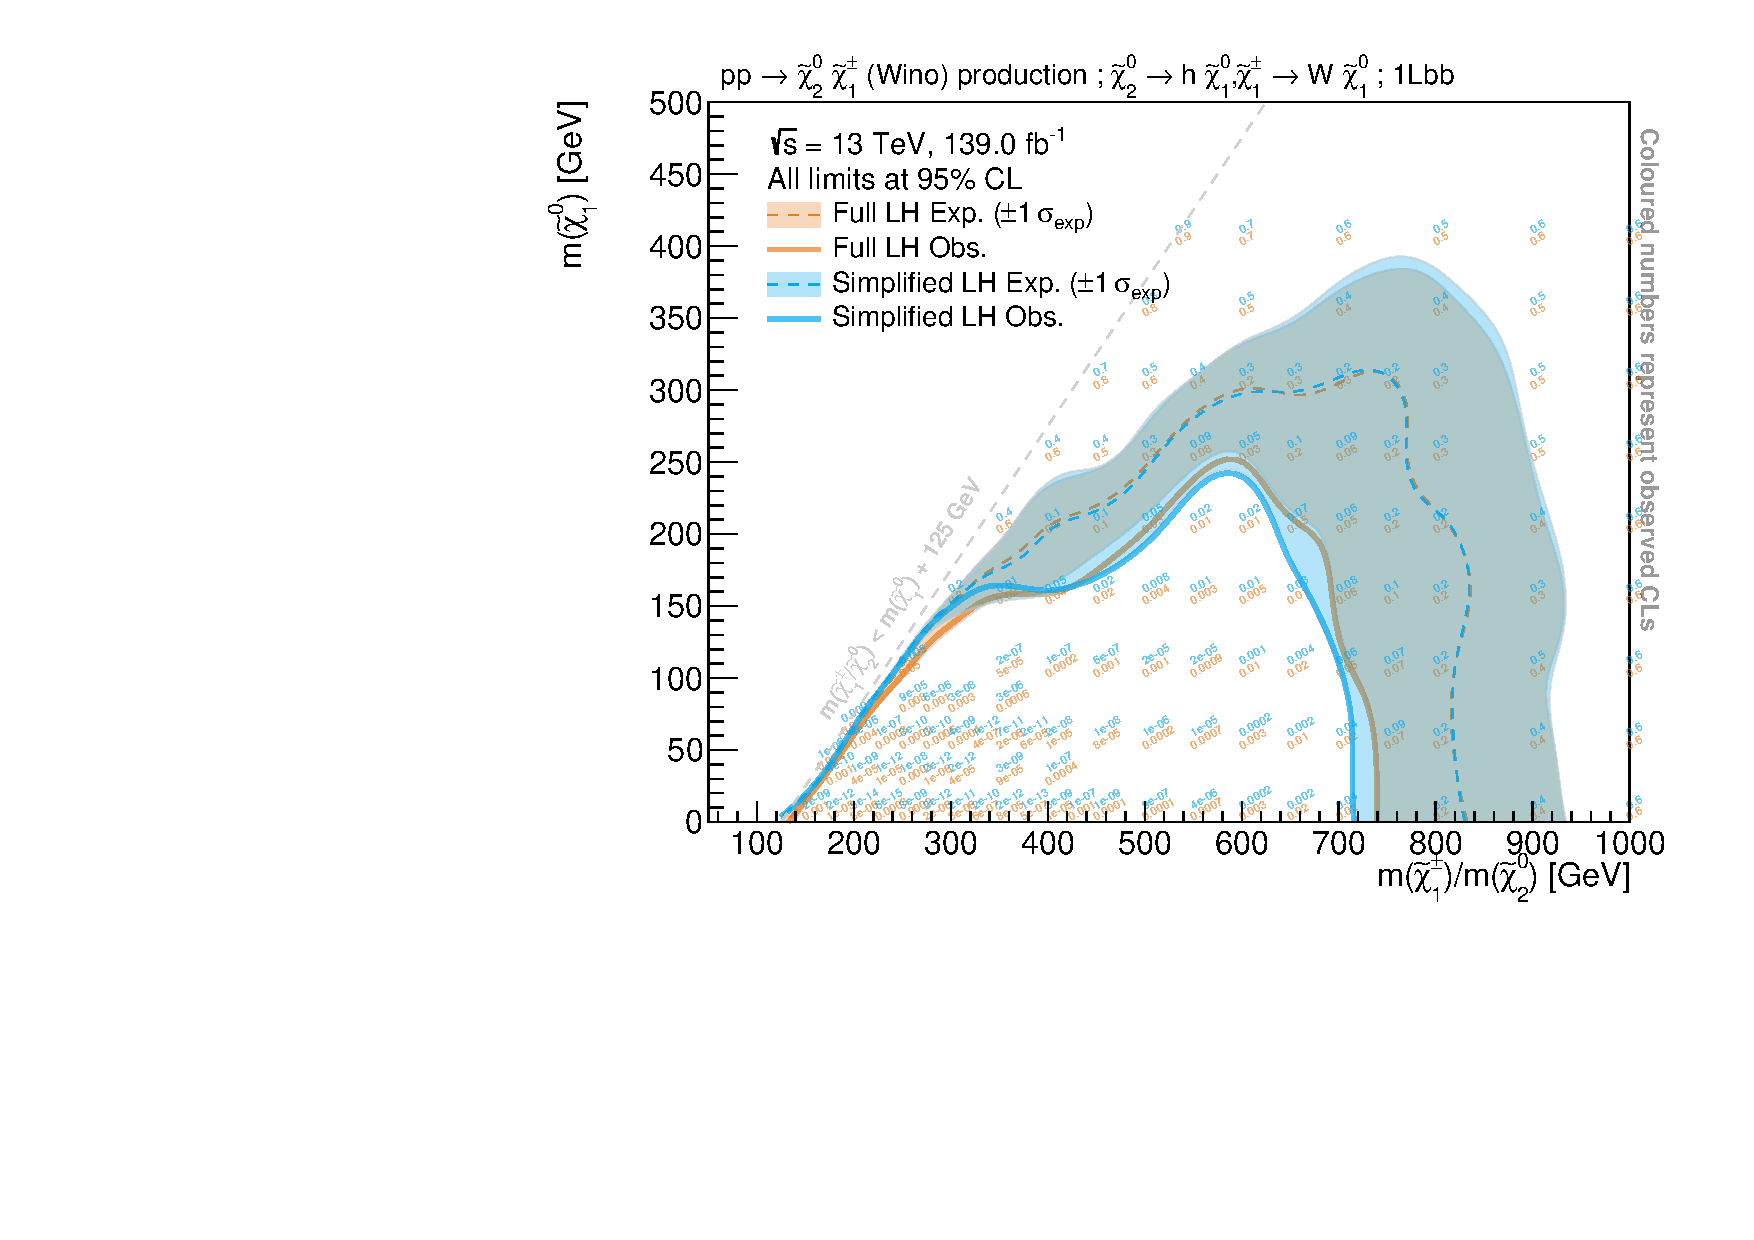
\includegraphics[width=0.60\textwidth]{exclusion_1Lbb_CLs_noLabel}}
\end{figure}



\begin{figure}
	\centering
	\begin{subfigure}[b]{0.5\textwidth}
		\centering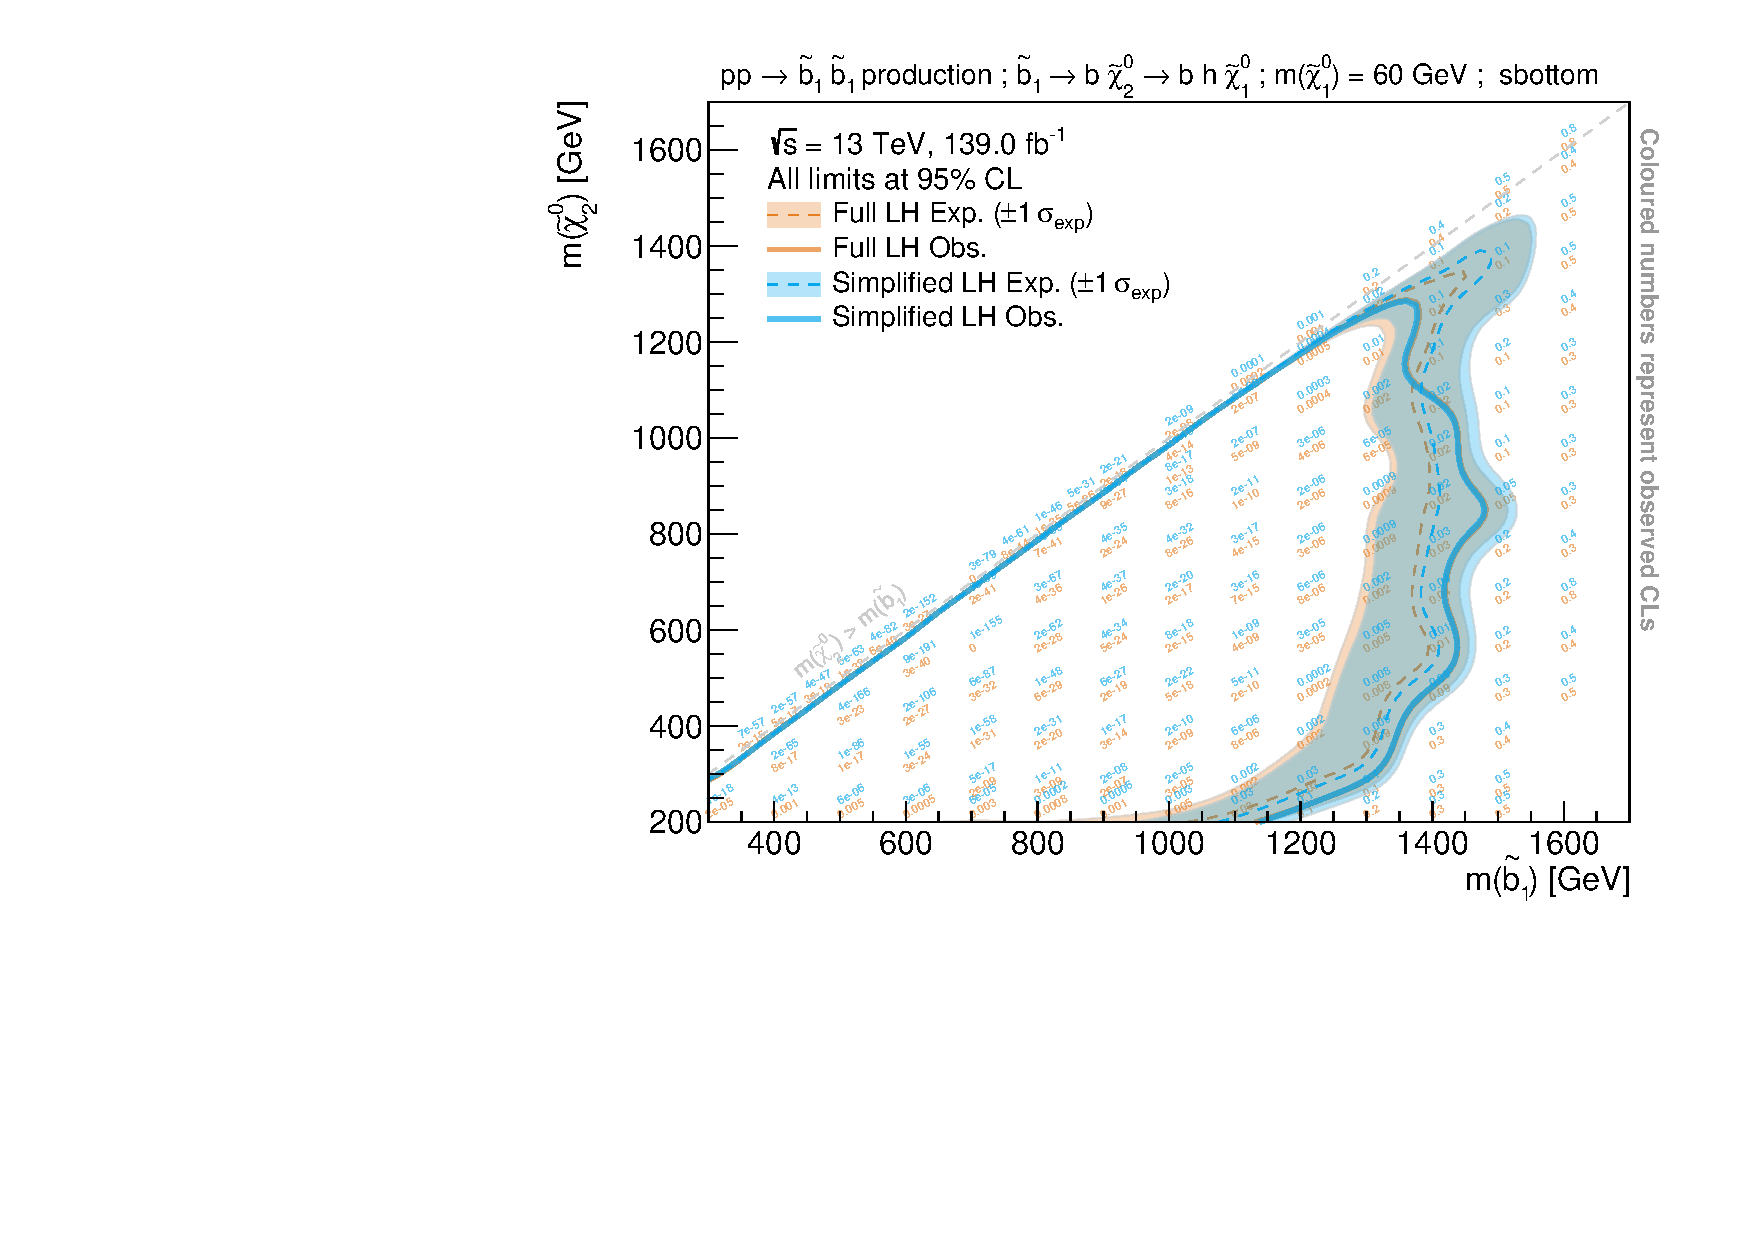
\includegraphics[width=\textwidth]{exclusion_sbottom_CLs_noLabel}
		\caption{ATLAS sbottom search~\cite{SUSY-2018-31}\label{fig:results_sbottom}}
	\end{subfigure}\hfill
	\begin{subfigure}[b]{0.5\textwidth}
		\centering\includegraphics[width=\textwidth]{exclusion_stop1L_CLs_noLabel}
		\caption{ATLAS stop search\label{fig:results_stop1L}}
	\end{subfigure}\hfill
	\begin{subfigure}[b]{0.5\textwidth}
		\centering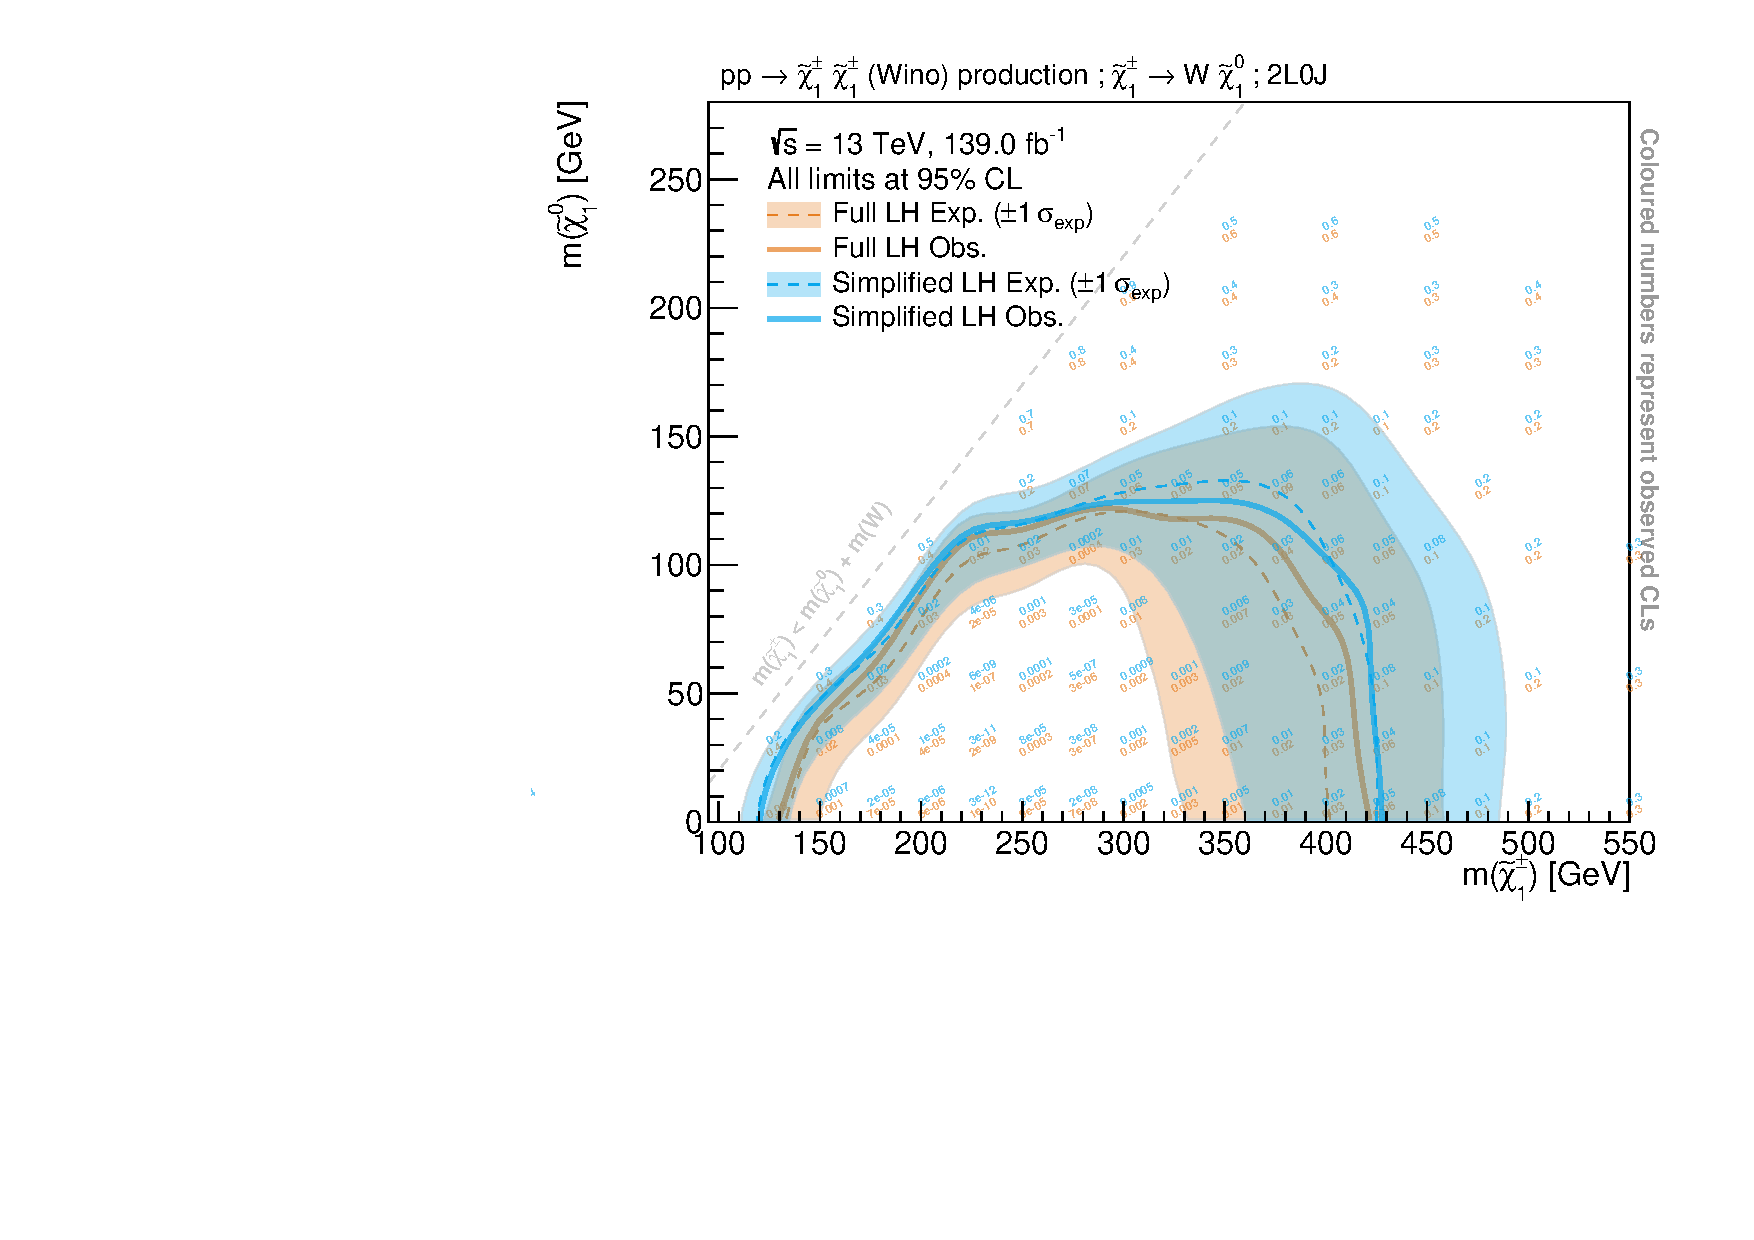
\includegraphics[width=\textwidth]{exclusion_2L0J_CLs_noLabel}
		\caption{ATLAS 2-lepton search~\cite{SUSY-2018-32}\label{fig:results_2L0J}}
	\end{subfigure}\hfill
	\begin{subfigure}[b]{0.5\textwidth}
		\centering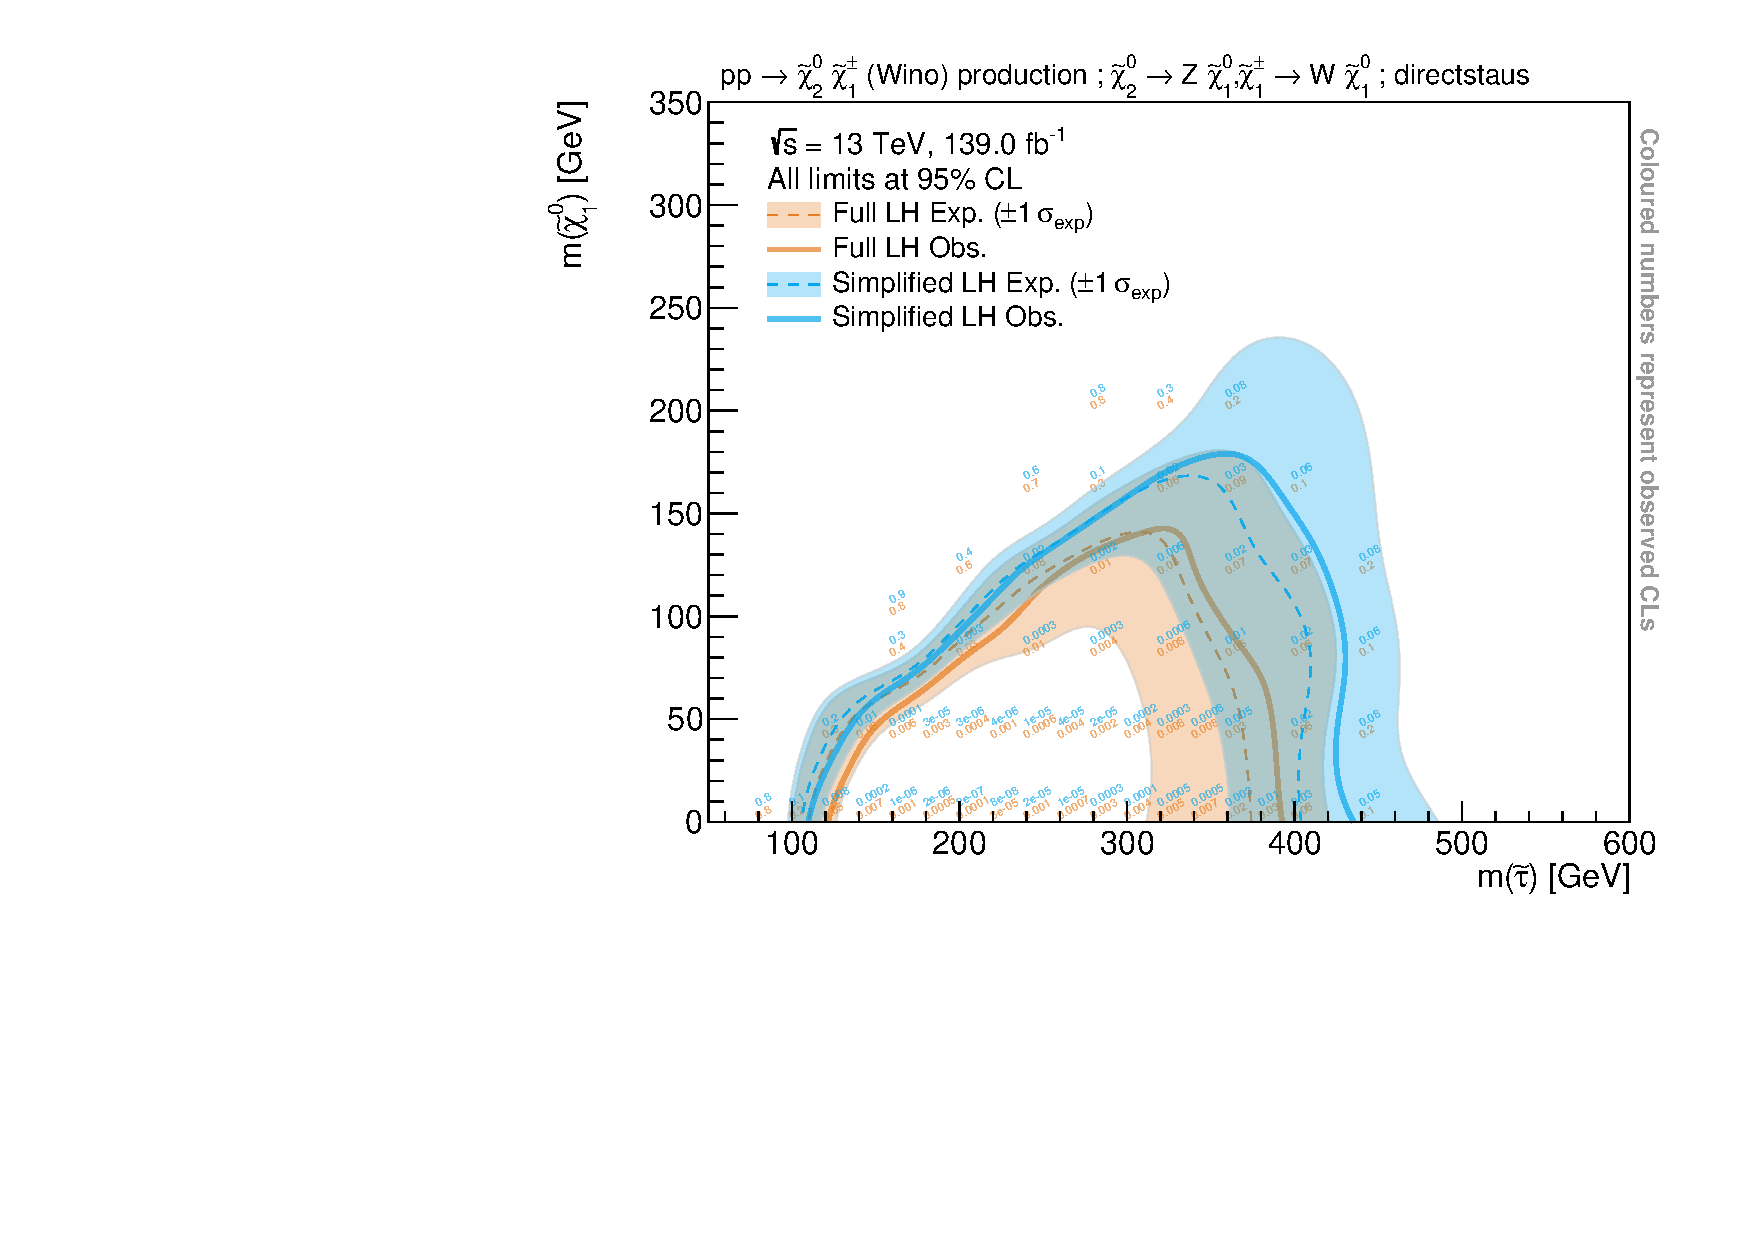
\includegraphics[width=\textwidth]{exclusion_directstaus_CLs_noLabel}
		\caption{ATLAS direct stau search~\cite{SUSY-2018-04}\label{fig:results_directstaus}}
	\end{subfigure}\hfill
	\begin{subfigure}[b]{0.5\textwidth}
		\centering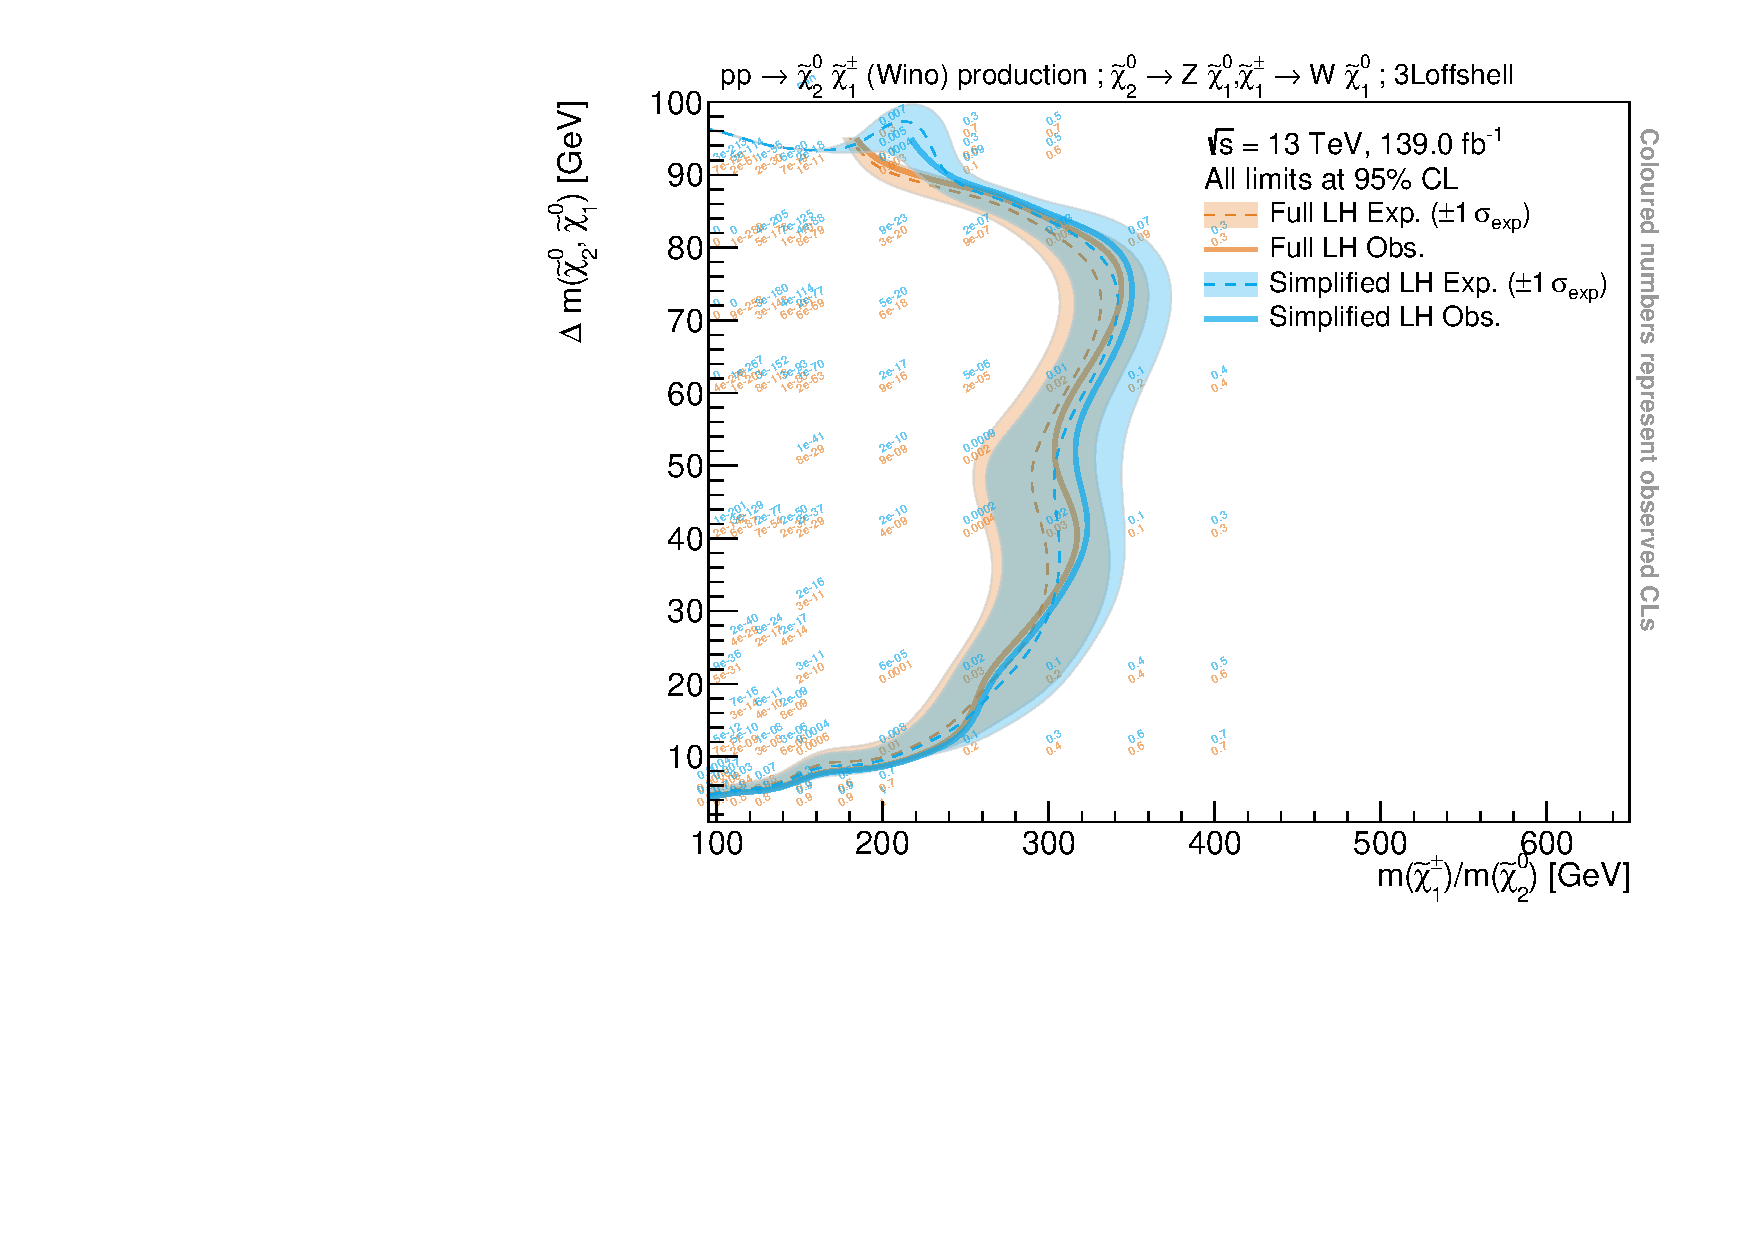
\includegraphics[width=\textwidth]{exclusion_3Loffshell_CLs_noLabel}
		\caption{ATLAS 3-lepton search\label{fig:results_3Loffshell}}
	\end{subfigure}\hfill
	\begin{subfigure}[b]{0.5\textwidth}
		\centering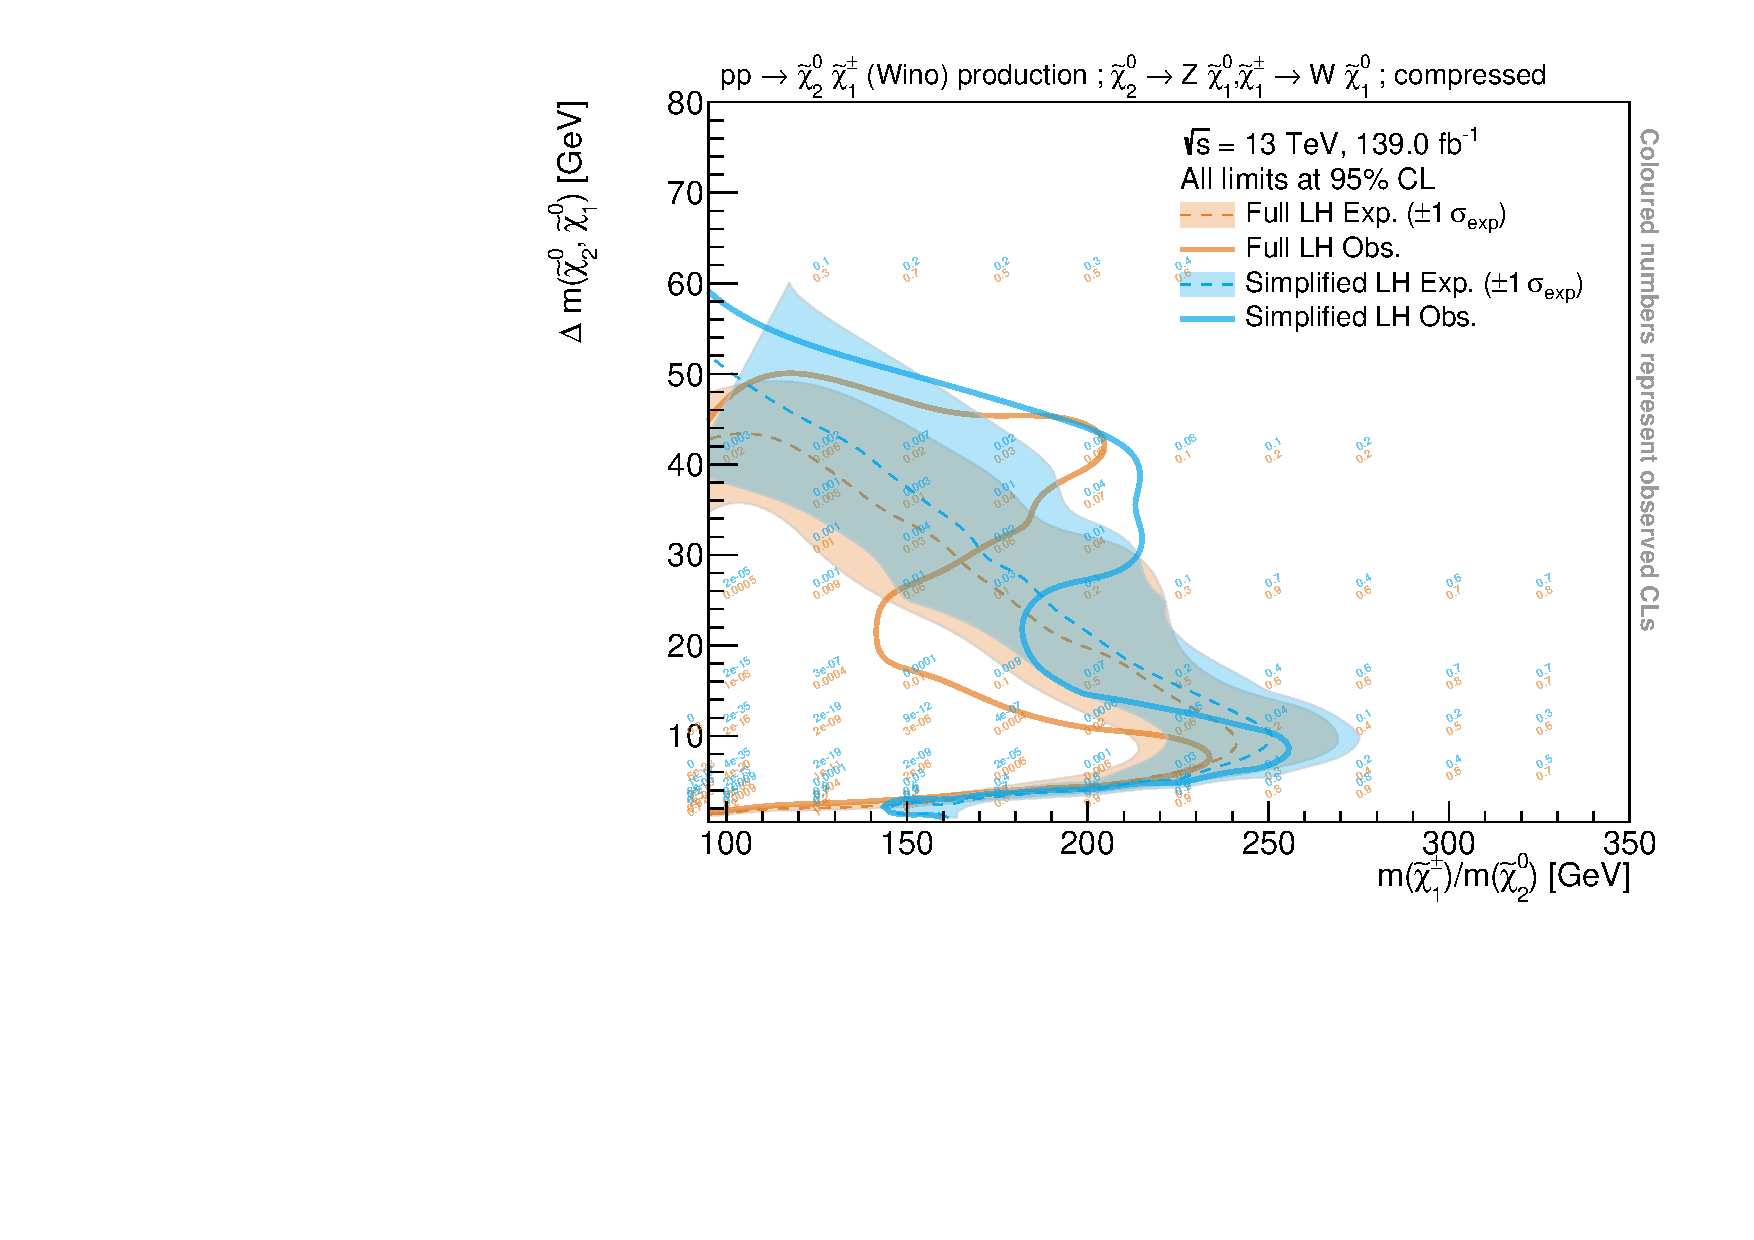
\includegraphics[width=\textwidth]{exclusion_compressed_CLs_noLabel}
		\caption{ATLAS compressed search~\cite{SUSY-2018-16}\label{fig:results_compressed}}
	\end{subfigure}\hfill
	\caption{Comparison of the simplified likelihood (blue contours) and full likelihood (orange contours) results for different ATLAS \gls{susy} searches. The observed contours are shown as solid lines, while the expected contours are shown as dashed lines. Observed CL$_s$ values from both likelihoods are given. The uncertainty band includes all \gls{mc} statistical and systematic uncertainties in the case of the full likelihood, and the simplified uncertainties in the case of the simplified likelihood.}\label{fig:results_analyses}
\end{figure}



\begin{figure}
	\centering
	\begin{subfigure}[b]{0.5\textwidth}
		\centering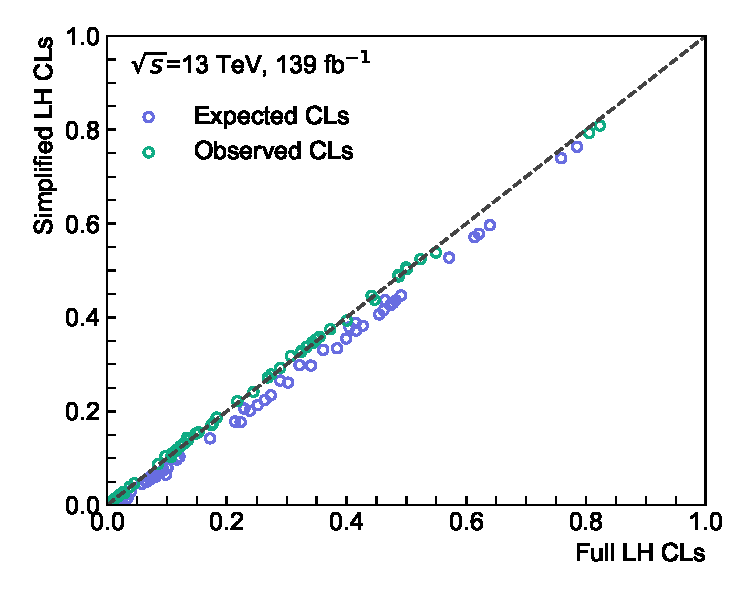
\includegraphics[width=\textwidth]{cls_scatter_sbottom_lin}
		\caption{ATLAS sbottom search~\cite{SUSY-2018-31}}
	\end{subfigure}\hfill
	\begin{subfigure}[b]{0.5\textwidth}
		\centering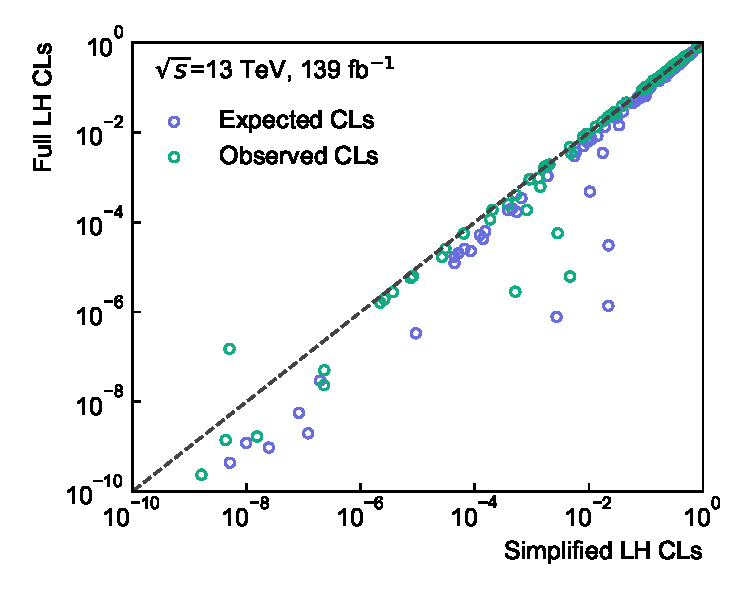
\includegraphics[width=\textwidth]{cls_scatter_sbottom_log}
		\caption{ATLAS sbottom search~\cite{SUSY-2018-31}}
	\end{subfigure}\hfill
	\begin{subfigure}[b]{0.5\textwidth}
		\centering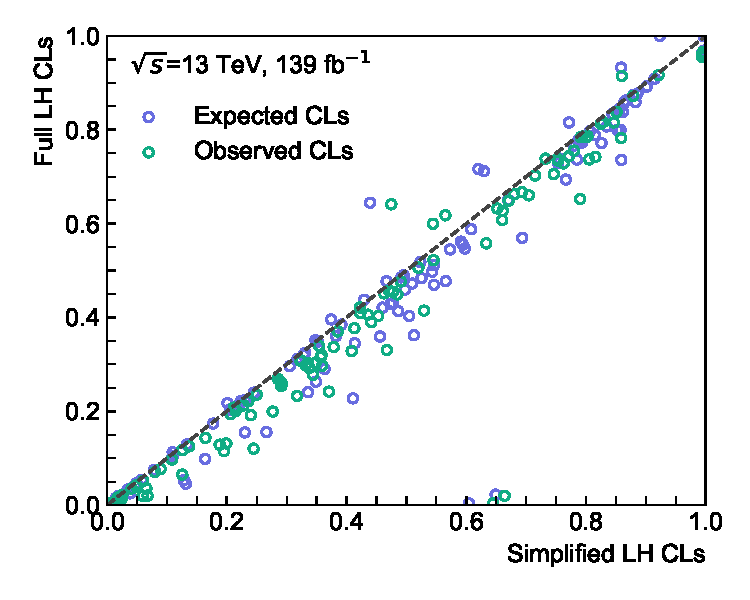
\includegraphics[width=\textwidth]{cls_scatter_stop1L_lin}
	\caption{ATLAS stop search}
	\end{subfigure}\hfill
	\begin{subfigure}[b]{0.5\textwidth}
		\centering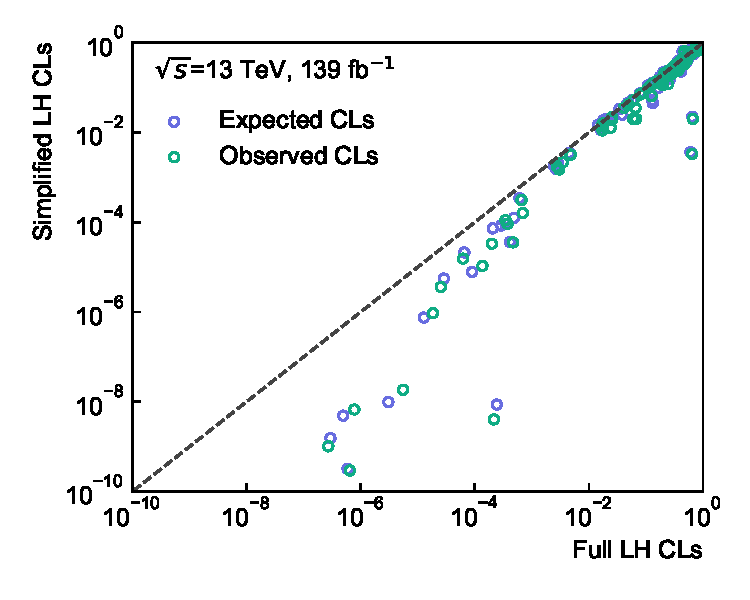
\includegraphics[width=\textwidth]{cls_scatter_stop1L_log}
		\caption{ATLAS stop search}
	\end{subfigure}\hfill
	\begin{subfigure}[b]{0.5\textwidth}
		\centering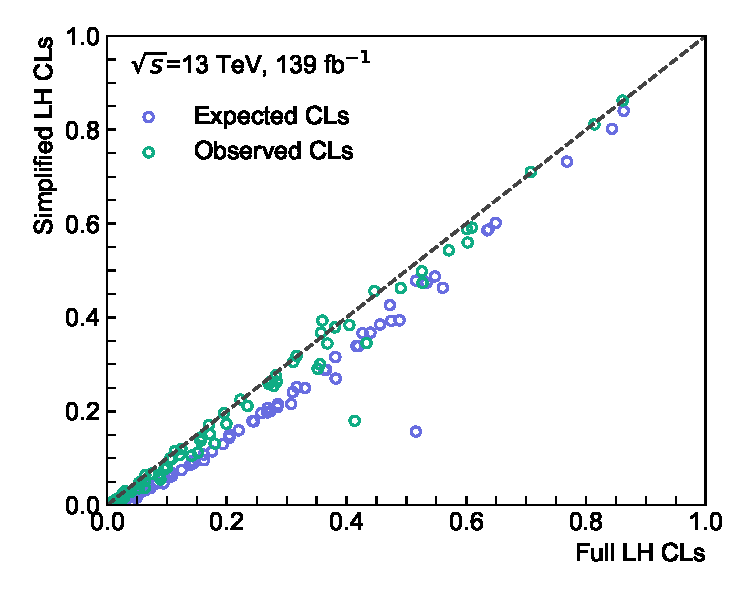
\includegraphics[width=\textwidth]{cls_scatter_2L0J_lin}
		\caption{ATLAS 2-lepton search~\cite{SUSY-2018-32}}
	\end{subfigure}\hfill
	\begin{subfigure}[b]{0.5\textwidth}
		\centering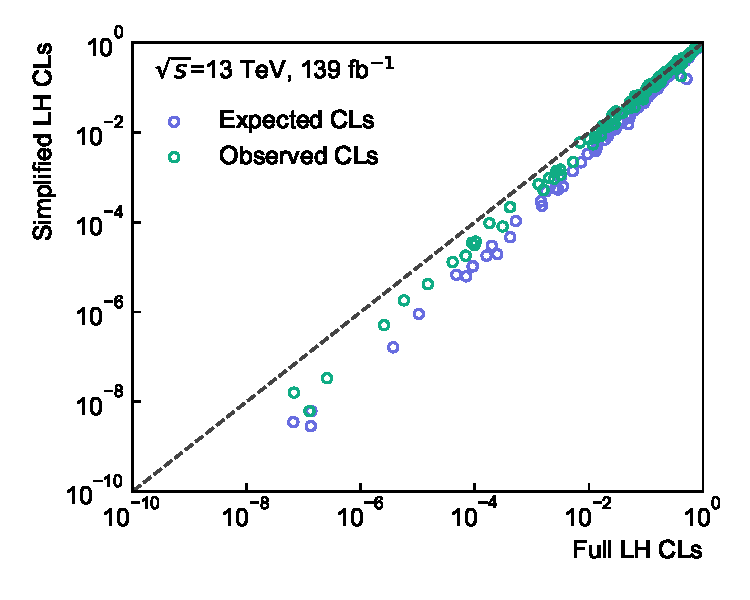
\includegraphics[width=\textwidth]{cls_scatter_2L0J_log}
		\caption{ATLAS 2-lepton search~\cite{SUSY-2018-32}}
	\end{subfigure}\hfill
	\caption{Scatter plots comparing the observed and expected CL$_s$ values obtained using the simplified and the full likelihoods for the same set of signal models originally considered in the various ATLAS \gls{susy} searches. Both linear and logarithmic scale representations are shown on the left- and right-hand side, respectively, illustrating the full range of CL$_s$ values. Apart from the scales, both columns show exactly the same results for each row of plots.}\label{fig:app_results_cls_1}
\end{figure}


\begin{figure}
	\centering
	\begin{subfigure}[b]{0.5\textwidth}
		\centering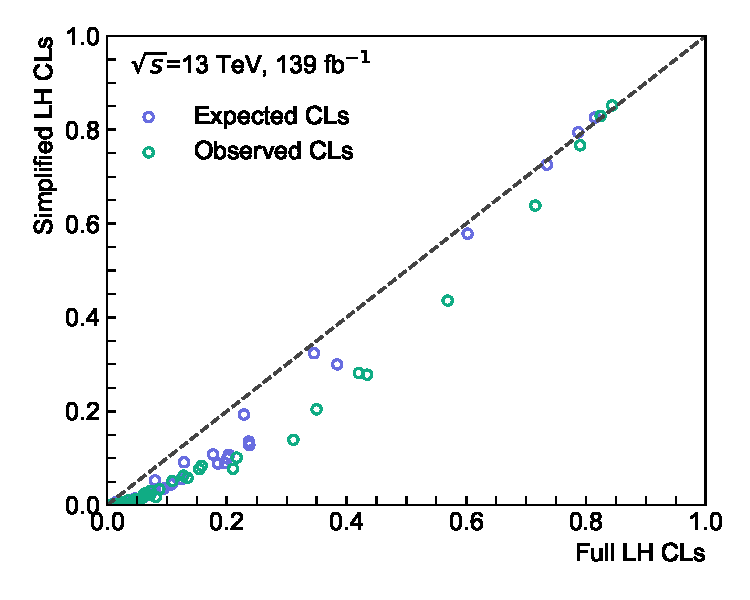
\includegraphics[width=\textwidth]{cls_scatter_directstaus_lin}
		\caption{ATLAS direct stau search~\cite{SUSY-2018-04}}
	\end{subfigure}\hfill
	\begin{subfigure}[b]{0.5\textwidth}
		\centering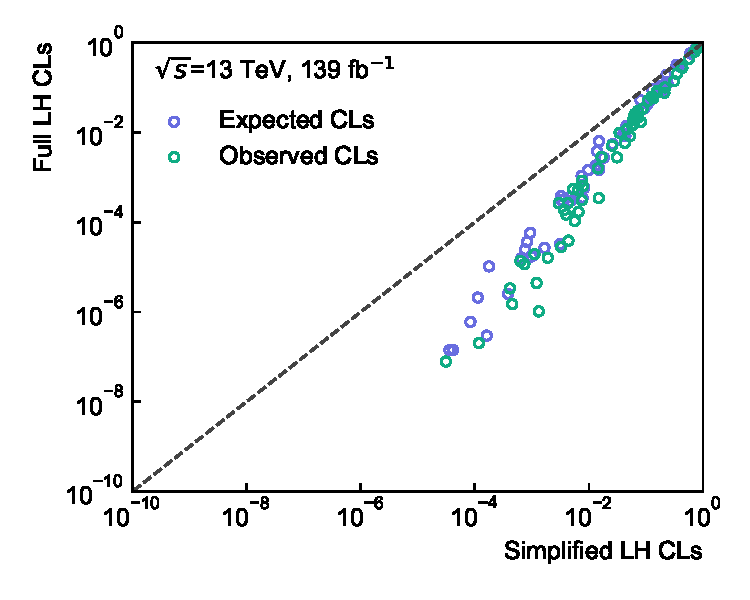
\includegraphics[width=\textwidth]{cls_scatter_directstaus_log}
		\caption{ATLAS direct stau search~\cite{SUSY-2018-04}}
	\end{subfigure}\hfill
	\begin{subfigure}[b]{0.5\textwidth}
		\centering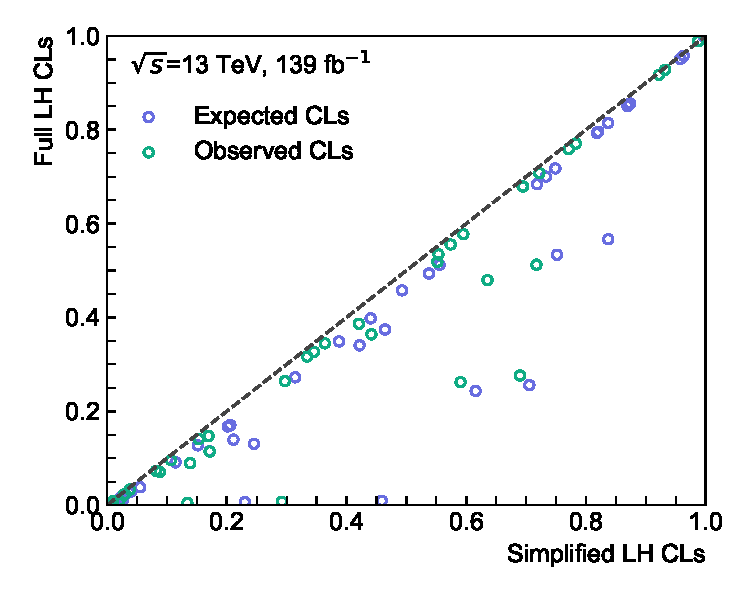
\includegraphics[width=\textwidth]{cls_scatter_3Loffshell_lin}
		\caption{ATLAS 3-lepton search}
	\end{subfigure}\hfill
	\begin{subfigure}[b]{0.5\textwidth}
		\centering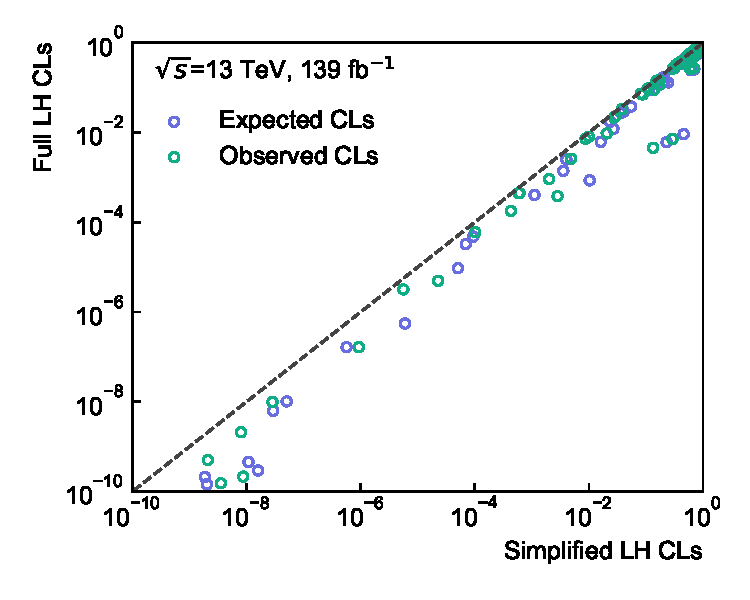
\includegraphics[width=\textwidth]{cls_scatter_3Loffshell_log}
		\caption{ATLAS 3-lepton search}
	\end{subfigure}\hfill
	\begin{subfigure}[b]{0.5\textwidth}
		\centering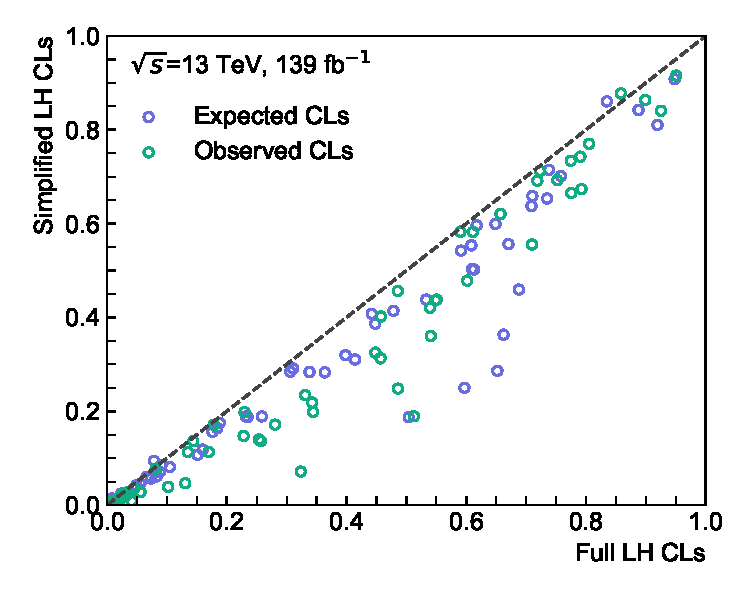
\includegraphics[width=\textwidth]{cls_scatter_compressed_lin}
		\caption{ATLAS compressed search~\cite{SUSY-2018-16}}
	\end{subfigure}\hfill
	\begin{subfigure}[b]{0.5\textwidth}
		\centering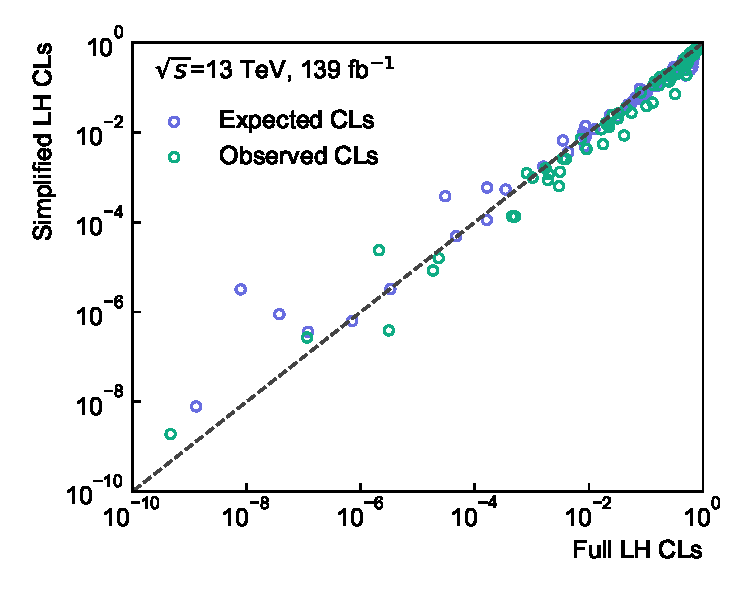
\includegraphics[width=\textwidth]{cls_scatter_compressed_log}
		\caption{ATLAS compressed search~\cite{SUSY-2018-16}}
	\end{subfigure}\hfill
	\caption{Scatter plots comparing the observed and expected CL$_s$ values obtained using the simplified and the full likelihoods for the same set of signal models originally considered in the various ATLAS \gls{susy} searches. Both linear and logarithmic scale representations are shown on the left- and right-hand side, respectively, illustrating the full range of CL$_s$ values. Apart from the scales, both columns show exactly the same results for each row of plots.}\label{fig:app_results_cls_2}
\end{figure}